\section{Experimental Results}
\label{sec:results}

In this section we analyze the results with the combination of CMS
data, the statistical model forecasts and in situ observations to
assess the impact to short-term ocean prediction in a dynamic coastal
environment like \naze.

Fig. \ref{fig:sst} provides an overview of the environmental
conditions observed during the three-day experimental window
considered in this study
(29\textsuperscript{th}–-31\textsuperscript{st} October). The
background fields correspond to the Level-3 Sea Surface Temperature
(SST) product from CMS. The operational area was compact, covering
approximately 100 km\textsuperscript{2} south of the \naz Canyon.
While all missions were planned using the sampling algorithm to
explore temperature variability predicted by the statistical model, on
31\textsuperscript{st} October, XP2 followed a cross-shore transect of
approximately 13 km to sample an internal wave hotspot; for the
purpose of this study, it serves as an independent ground-truth
dataset. \kcomment{Not sure I understand. Above the reference is for
  the op area being south of the canyon. So what was the intent to
  send XP2 and how is it fitting into the op area (or not)? This para
  could do with some clarity.}
These observations are thus used as a reference for
evaluating the forecast cases \textbf{C1-–C4} and \textbf{D1–-D4}.

During this period, the coastal ocean was influenced by a late-season
upwelling–relaxation cycle. At the beginning of the sequence
(29\textsuperscript{th} October), the SST field reveals the
characteristic signature of coastal upwelling, with colder water
masses extending offshore due to wind-driven Ekman transport that
brings subsurface, nutrient-rich waters to the surface. In the
following days, the weakening of upwelling-favorable winds led to a
relaxation phase, during which warmer offshore waters gradually
advanced toward the coast. This transition is reflected in the SST
maps by an overall warming trend in the nearshore region, particularly
evident on 1\textsuperscript{st} November (Fig. \ref{fig:sst}).

It is important to note that the SST imagery is partially affected by
cloud coverage, which limits the availability and accuracy of
satellite-derived temperature data. These gaps arise from the
radiometric constraints of indirect SST retrieval, resulting in
reduced spatial continuity and increased uncertainty near cloudy
regions.  Despite these limitations, the SST patterns clearly capture
the dominant mesoscale features and coastal processes driving the
observed variability during the experiment.
% These evolving conditions provided a natural setting for testing the
% adaptive sampling and data assimilation framework.  
The pronounced temperature gradients associated with the upwelling
front generated well-defined spatial and temporal variability,
allowing the evaluation of how targeted in-situ observations can
improve the predictive skill of the statistical model in a coastal
environment.


\begin{figure}
  \centering 

  \subfigure[Sea surface temperature (SST) and XP2, XP3 and XP5
  trajectories during the \proj experiment
  (29\textsuperscript{th}-–31\textsuperscript{st} October)
  \rmcomment{ADD new subfigure november}.]
  {\label{fig:sst}\includegraphics[width=1\linewidth]{fig/Figure_sst_auv_l3_zoom.pdf}}

  \subfigure[Time–-depth temperature evolution observed by XP2, XP3,
  and XP5 during the \proj experiment
  (29\textsuperscript{th}–-31\textsuperscript{st} October).]
  {\label{fig:temperatureprofiles}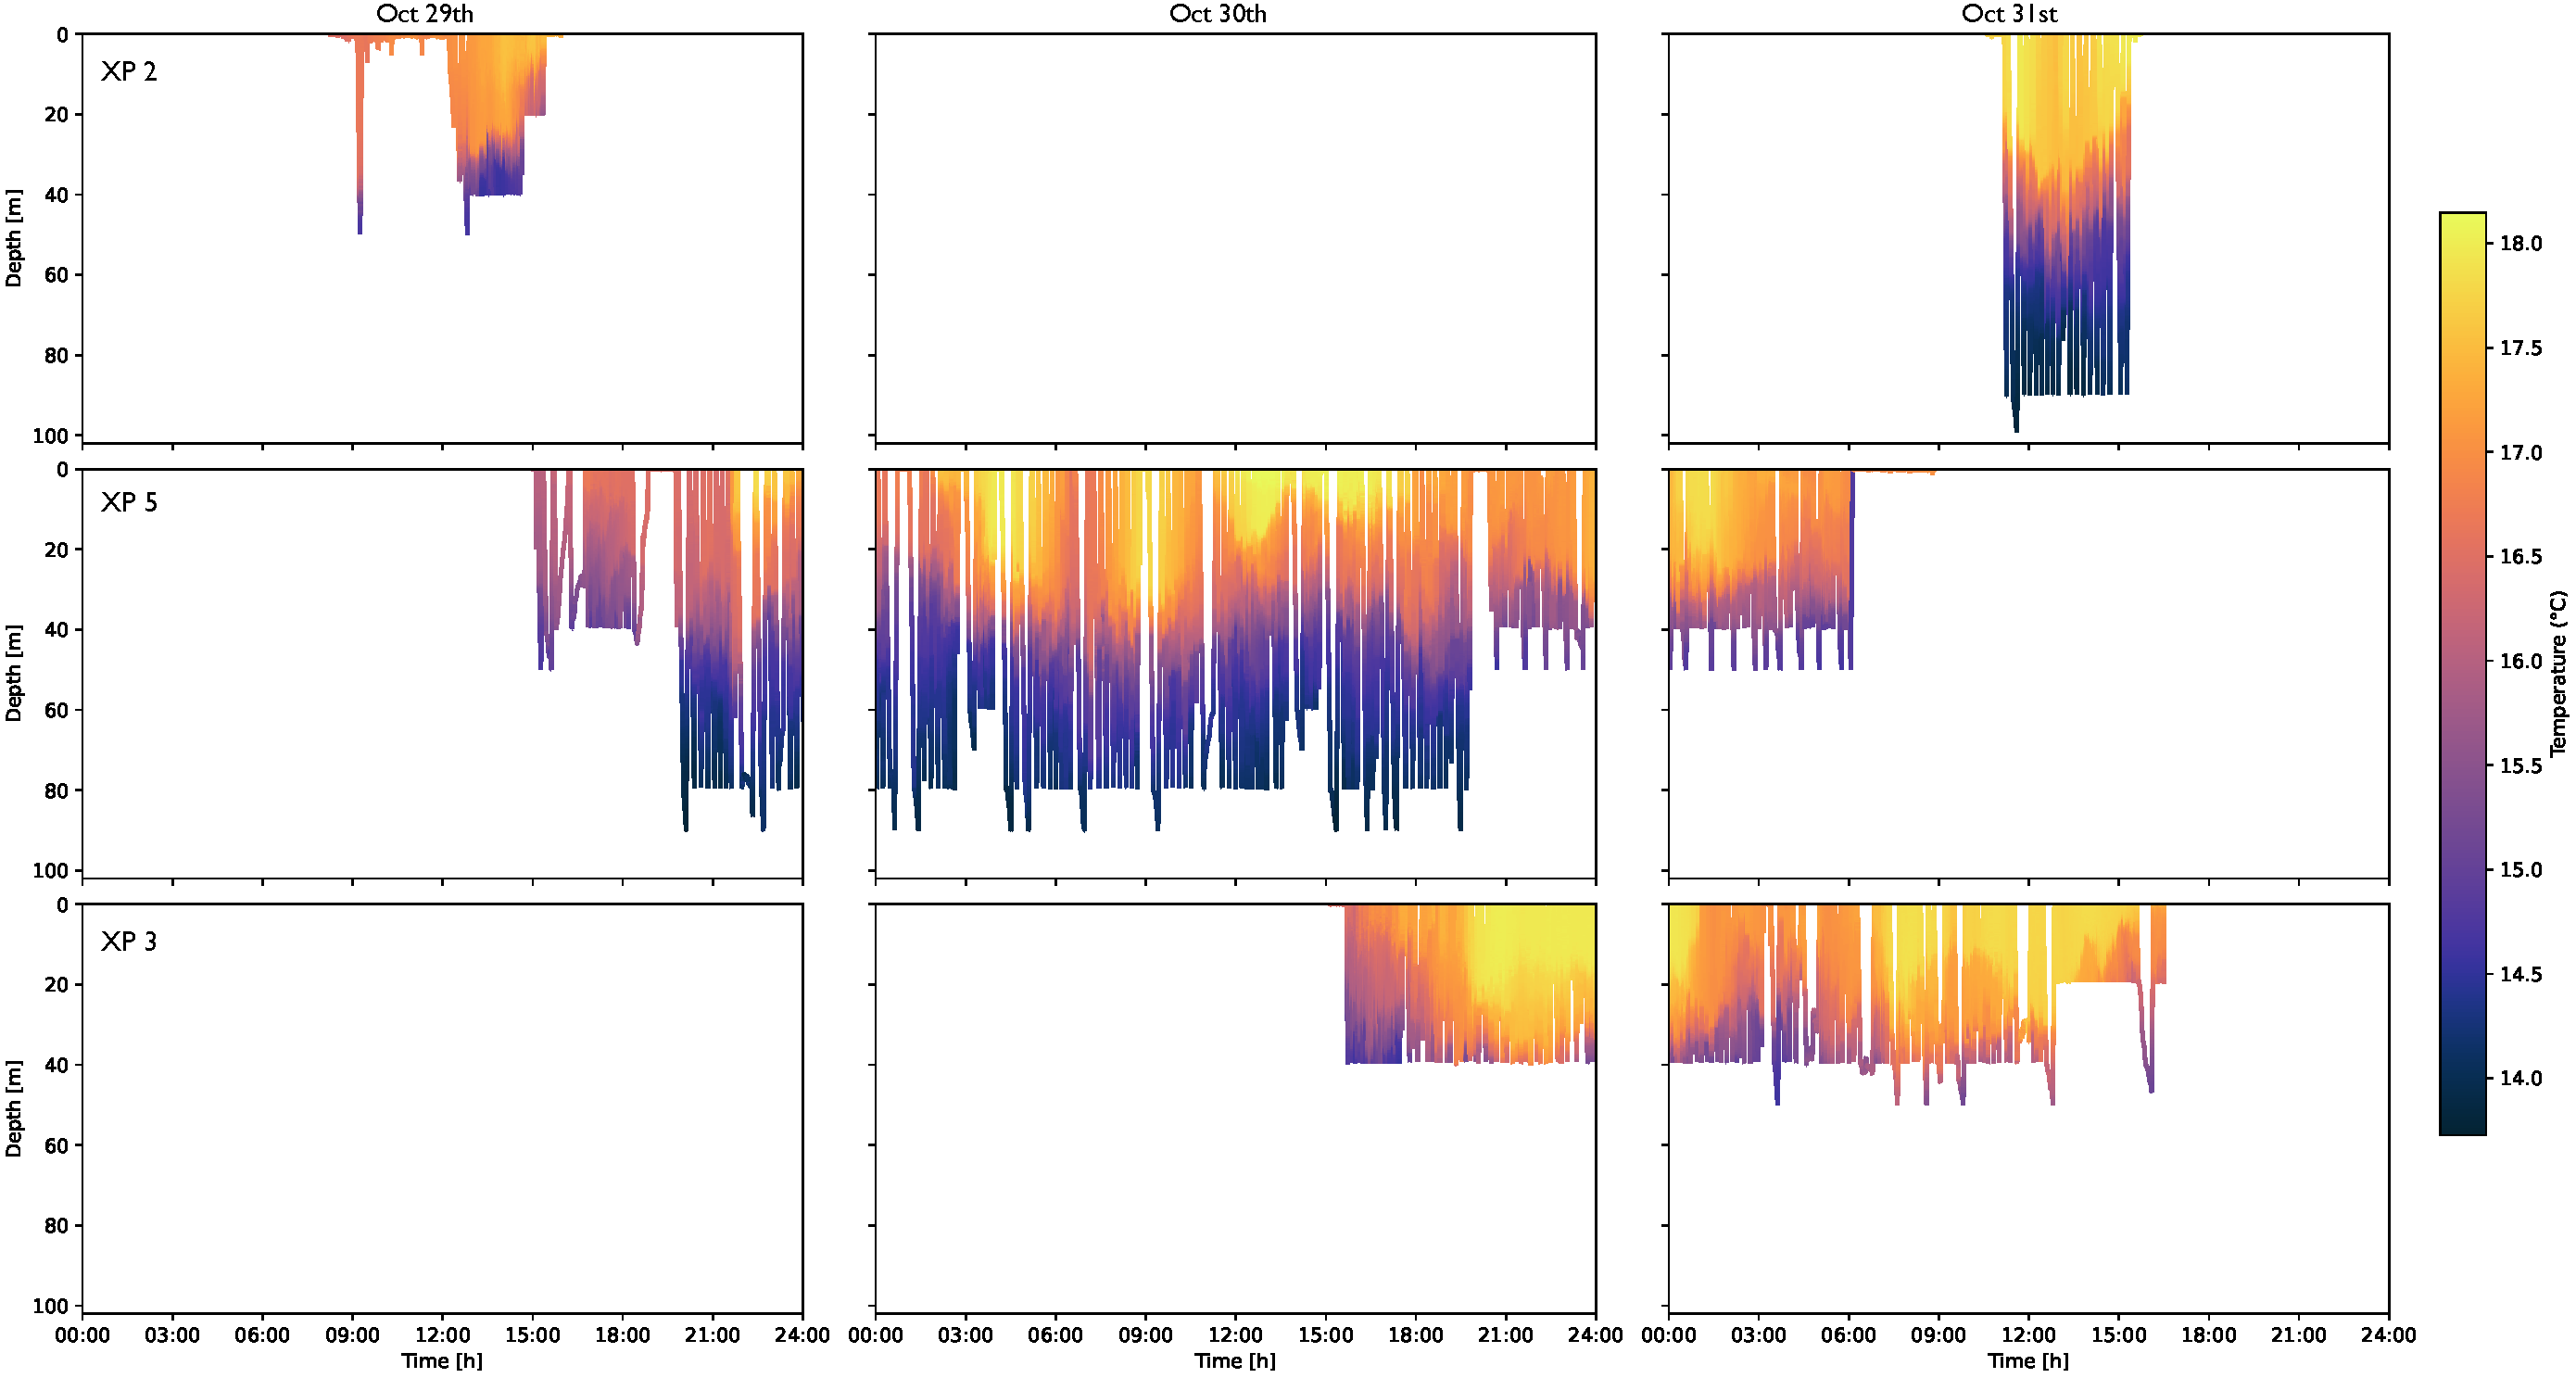
\includegraphics[width=1\linewidth]{fig/Figure2_100m.pdf}}
  \caption{}
\end{figure}

Fig.\ref{fig:temperatureprofiles} presents the vertical temperature
distribution recorded by the AUVs during their respective missions
between 29\textsuperscript{th} and 31\textsuperscript{st} October. The
panels show temperature as a function of time and depth, illustrating
the temporal and vertical structure of the coastal water column
throughout the three-day experimental sequence, as well as
highlighting the non-linear nature of field logistics in multi-vehicle
operations, where dynamic scheduling, resource allocation, and
environmental constraints determine the actual temporal coverage of
the missions.

XP2 operated on 29\textsuperscript{th} October, XP5 on
29\textsuperscript{th}, 30\textsuperscript{th}, and
31\textsuperscript{st} October, and XP3 on 30\textsuperscript{th} and
31\textsuperscript{st} October.
% However, this depth range was not
% always achieved due to logistical and bathymetric constraints.
The temperature fields reveal a thermocline and a progressive warming
of the surface layer down to approximately 40m depth, with
temperatures ranging from around 14$^{\circ}$C in deeper layers to
about 18$^{\circ}$C near the surface, reaching their maximum on
30\textsuperscript{th} October afternoon during XP5’s mission.

% It is important to note that the trajectories shown in the previous
% figure might suggest that the AUVs remained continuously at sea for 24
% hours each day. However, as Fig. \ref{fig:temperatureprofiles}
% demonstrates, this was not the case. The vehicles can be deployed and
% recovered multiple times per day, with operational windows limited by
% logistics, weather, and available support assets. This figure,

\subsection{Data Evaluation}

The following section summarizes the quantitative evaluation of the
model’s predictive performance across all tested scenarios. Fig.
\ref{fig:rms_ABB1}, \ref{fig:rms_c}, and \ref{fig:rms_d} present the
RMSE between the statistical model forecasts and the in situ
temperature observations collected by the AUVs. These figures cover
all experimental configurations examined in this study. % providing a
% comprehensive overview of how the assimilation of targeted AUV data
% affects the model’s short-term forecast accuracy and vertical
% consistency.

\begin{wrapfigure}{!h}{2.75in}
  \centering
  \includegraphics[scale=0.5]{fig/rms_ABB1.png}
  \caption{Root Mean Square Error (RMSE) (in $^{\circ}$C) between
    statistical model forecasts and in situ AUV temperature
    observations for 29\textsuperscript{th}–-30\textsuperscript{st}
    October. Scenario \textbf{A} corresponds to the baseline
    statistical forecast generated based on CMS data up to
    29\textsuperscript{th} October. Scenarios \textbf{B} and
    \textbf{B1} represent forecasts for 30\textsuperscript{th} October
    without and with the assimilation of AUV observations collected by
    XP2, respectively. Values are shown for each depth level sampled
    during the missions.}
  \label{fig:rms_ABB1}
\end{wrapfigure}

% \kcomment{There were a number of typos in the following para. RM to
%   check that my fixes are accurate}

Fig. \ref{fig:rms_ABB1}, corresponds to the initial phase of the
experiments on the 29\textsuperscript{th} and the
30\textsuperscript{th}. Scenario \textbf{A} represents the baseline
statistical forecast based on CMS data. The \textbf{B} and \textbf{B1}
scenarios correspond to forecasts for 30\textsuperscript{th} October
without and with the assimilation of in situ observations during the
previous day.  Across the vertical profile, RMSE values in scenario
\textbf{A} range from approximately 0.48$^{\circ}$C near the surface
to 1.33$^{\circ}$C at 40m, with a mean RMSE of about
0.74$^{\circ}$C. The errors increase with depth, indicating reduced
model skill in reproducing the subsurface thermal structure.  The
non-assimilated \textbf{B} scenario remains similar to \textbf{A} in
the upper layers but diverges below 20m. After assimilation, the
\textbf{B1} case shows a consistent improvement throughout the column
compared to the non-assimilated \textbf{B} scenario, with RMSE values
between 0.31$^{\circ}$C and 0.55$^{\circ}$C and an average of
0.39$^{\circ}$C, representing an overall reduction of nearly 50\%
relative to \textbf{B}. This improvement is most pronounced in the
5–-20m layers, coinciding with the strongest vertical temperature
gradients and the region most densely sampled by the AUVs, and in turn
confirming that the assimilation of recent AUV data substantially
improves the short-term forecast skill and internal consistency of the
model.

The results for 31\textsuperscript{st} October, summarized in
Fig. \ref{fig:rms}, correspond to the phase of the experiment in which
multiple assimilation scenarios were tested. The \textbf{C}-series
uses CMS data up to 30\textsuperscript{th} October, whereas the
\textbf{D}-series uses CMS up to 29\textsuperscript{th} October,
representing a less favorable statistical initial state. In both
cases, the assimilation scenarios (\textbf{C1-–C4} and
\textbf{D1-–D4}) correspond to the incorporation of AUV data collected
during the previous days.

A consistent reduction in statistical forecast error is observed
across most vehicles and assimilation stages. In the
\textbf{C}-series, the average RMSE across all AUVs decreases from
approximately 0.40$^{\circ}$C in \textbf{C} to 0.31$^{\circ}$C in
\textbf{C4}, while in the \textbf{D}-series, the mean RMSE drops from
0.55$^{\circ}$C in \textbf{D} to 0.40$^{\circ}$C in
\textbf{D4}. These improvements correspond to an average error
reduction of 25–-30\%, demonstrating that the assimilation of targeted
observations can compensate for differences in the initial state and
improve predictive accuracy.

It should be noted, however, that the improvement is not uniform
across all vehicles. For XP3 and XP5, which performed targeted
sampling in the same area where previous assimilation data were
collected, RMSE values show a clear reduction. In contrast, XP2, which
on 31\textsuperscript{st} October performed an independent cross-shore
transect outside the main target region, exhibits a weaker response to
assimilation. The implications of this behavior and its relevance for
evaluating the predictive robustness of the framework are examined in
the Section \ref{sec:disc}.  Vertically, RMSE profiles show similar
behavior in both experiment sets: errors tend to increase gradually
below 25–30m, where model uncertainty and unresolved variability are
higher. However, this gradient weakens considerably in the fully
assimilated cases (\textbf{C4} and \textbf{D4}), particularly in the
upper 30m, where the assimilation of prior AUV data significantly
improves the representation of the temperature structure and
short-term thermal evolution probably associated with the
upwelling–relaxation transition.


\begin{figure}
  \centering 

  \subfigure[RMSE (in $^{\circ}$C) between statistical model forecasts
  and in situ AUV temperature measurements for 31\textsuperscript{st}
  October, scenarios \textbf{C}, \textbf{C1-–C4}. The forecasts were
  initialized using CMS data available up to 30\textsuperscript{th}
  October, and the assimilation steps progressively include AUV data
  collected on previous days. Results are presented for each vehicle
  individually and for the combined dataset (all AUVs).]
  {\label{fig:rms_c}\includegraphics[width=1\linewidth]{fig/rms_c.png}}

  \subfigure[RMSE (in $^{\circ}$C) between statistical model forecasts
  and in situ AUV temperature measurements for 31\textsuperscript{st}
  October, scenarios \textbf{D}, \textbf{D1-–D4}. The forecasts were
  initialized using CMS data available up to 30\textsuperscript{th}
  October, and the assimilation steps progressively include AUV data
  collected on previous days. Results are presented for each vehicle
  individually and for the combined dataset (all AUVs).]
  {\label{fig:rms_d}\includegraphics[width=1\linewidth]{fig/rms_d.png}}
  \caption{}
  \label{fig:rms}
  % above is necessary to get the figure numbering right.
\end{figure}

To further interpret the RMSE results presented in Fig. \ref{fig:rms},
Fig. \ref{fig:scatter} focuses on the most contrasted scenarios: the
baseline cases without assimilation (\textbf{C} and \textbf{D}) and
those incorporating the full set of AUV observations from previous
days (\textbf{C4} and \textbf{D4}). This comparison illustrates the
model's ability to reproduce the observed temperatures at each
measurement point accurately, contrasting the non-assimilated cases
(\textbf{C} and \textbf{D}) with the partially and fully assimilated
ones (\textbf{C1-4} and \textbf{D1-4}). 

The four scatter plots compare the measurements acquired in situ on
31\textsuperscript{st} October against the corresponding
geostatistical predictions derived under each scenario. The
observations include all available measurements collected along the
missions on that day (see Fig. \ref{fig:sst} and
\ref{fig:temperatureprofiles}. Colors indicate the depth layers
associated with the vertical discretization used in the deterministic
CMS model which defines the vertical structure of the statistical
model.

In the baseline scenarios without assimilation (\textbf{C} and
\textbf{D}), the plots exhibit a wide spread of points around the
reference line, indicating substantial discrepancies between the model
predictions and the observed AUV measurements. These deviations are
particularly evident in \kcomment{...,????} where surface temperatures
tend to be overestimated. This dispersion reflects the model’s limited
ability to accurately reproduce the vertical thermal structure when it
relies solely on CMS data without incorporating recent in situ
information.

In contrast, the fully assimilated scenarios (\textbf{C4} and
\textbf{D4}) show a much tighter clustering of points around the
reference, especially within the upper layers, where the previous AUV
missions provide dense and temporally relevant observations. This
reduction in spread suggests a clear improvement in predictive
accuracy, indicating that the assimilation of targeted measurements
effectively constrains the thermal structure and captures ongoing
physical transitions in the water column.

\begin{figure}[!]
  \centering
  \includegraphics[scale=0.7]{fig/scatter.png}
  \caption{Comparison between in situ AUV observations
    (31\textsuperscript{st} October) and geostatistical model
    predictions for scenarios \textbf{C}, \textbf{C4}, \textbf{D}, and
    \textbf{D4}. Shallower layers are shown in warmer colors (red to
    yellow), while deeper layers ($>$ 30m) are progressively
    represented in cooler shades (green to blue). The dashed red line
    provides a reference for perfect agreement.  \rmcomment{!not the
      final figure. need to correct and round values to 1 decimal
      place!}\kcomment{Also see my comment about making the scenarios
      into a Table instead of the text at the end of the methods
      section. If you have that table, it would be useful to have a
      copy of that same table highlighting the differences between the
      scenarios to make the figures (and text) more readable.}}
  \label{fig:scatter}
\end{figure}


